%%%%%%%%%%%%%%%%%%%%%%%%%%%%%%%%%%%%%%%%%%%%%%%%%%%%%%%%%%%%
%% INFORME DE LABORATORIO - UNIVERSIDAD MILITAR NUEVA GRANADA
%% PROGRAMA DE INGENIERÍA MECATRÓNICA
%% INFORME FINAL: ROBOT MÓVIL INTELIGENTE BASADO EN ESP32-S3
%%%%%%%%%%%%%%%%%%%%%%%%%%%%%%%%%%%%%%%%%%%%%%%%%%%%%%%%%%%%

\documentclass[journal]{IEEEtran}
\IEEEoverridecommandlockouts

%%%%%%%%%%%%%%%%%%%%%%%%%%%%%%
%%%% PAQUETES PRINCIPALES %%%%
%%%%%%%%%%%%%%%%%%%%%%%%%%%%%%
%% Orden: codificación e idioma -> figuras/tablas -> matemáticas ->
%% tikz -> hyperref al final (recomendado).
\usepackage[utf8]{inputenc}
\usepackage[T1]{fontenc}
\usepackage[spanish,es-tabla]{babel}
\usepackage{graphicx}
\usepackage{fancyhdr}
\usepackage{color}
\usepackage{xcolor}
\usepackage{wrapfig}
\usepackage{array}
\usepackage{multirow}
\usepackage{adjustbox}
\usepackage{amsmath}
\usepackage{nccmath}
\usepackage{amsfonts,latexsym}
\usepackage{enumerate}
\usepackage{booktabs}
\usepackage{float}
\usepackage{threeparttable}
\usepackage{array,colortbl}
\usepackage{ifpdf}
\usepackage{rotating}
\usepackage{cite}
%% stfloats es opcional (flotantes a dos columnas en el pie).
\IfFileExists{stfloats.sty}{\usepackage{stfloats}}{}
\usepackage{url}
\usepackage{listings}
\usepackage{makecell}
\usepackage{tikz}
\usetikzlibrary{arrows.meta,positioning,shapes.geometric,fit,calc}
%% hyperref se carga al final para evitar conflictos con el resto.
\usepackage{hyperref}

\setcellgapes{2pt}
\newcolumntype{P}[1]{>{\centering\arraybackslash}p{#1}}
\newcommand{\tabitem}{~~\llap{\textbullet}~~}
\newcommand{\ctt}{\centering\scriptsize\textbf}
\newcommand{\dtt}{\scriptsize\textbf}
\renewcommand\IEEEkeywordsname{Palabras clave}

\graphicspath{{../imagenes/}{../cad/}}

\hypersetup{
    colorlinks=true,
    linkcolor=black,
    citecolor=black,
    urlcolor=blue,
    pdftitle={Robot móvil inteligente basado en ESP32-S3},
    pdfauthor={Kevin Estivem Parra Oñate, Andres Felipe Escovedo Garzon, Camilo Santiago Alvarez Sierra}
}

\hyphenation{mi-cro-con-tro-la-dor co-mu-ni-ca-ción sen-so-res}

%%%%%%%%%%%%%%%%%%%%%%%%%%%%%%%%%%%%%%%%%%%%%%%%%%%%%%%%%%
%%%%%%%%%%% ENCABEZADO TIPO UMNG %%%%%%%%%%%%%%%%%%%%%%%%%
%%%%%%%%%%%%%%%%%%%%%%%%%%%%%%%%%%%%%%%%%%%%%%%%%%%%%%%%%%

\newcommand{\MYhead}{\smash{\scriptsize
\hfil\parbox[t][\height][t]{\textwidth}{\centering
\begin{picture}(0,0)
\put(-0,-17){\IfFileExists{LogoUMNG}{\includegraphics[width=27mm]{LogoUMNG}}{}}
\end{picture}
\hspace{5.4cm}
INFORME DE PROYECTO DE LABORATORIO
\hspace{3.5cm} Versión 2.0\\
\hspace{5.2cm}
PROGRAMA DE INGENIERÍA MECATRÓNICA
\hspace{3.0cm} Periodo 2026-2\\
\underline{\hspace{\textwidth}}}\hfil\hbox{}}}

\makeatletter
\def\ps@headings{%
\def\@oddhead{\MYhead}%
\def\@evenhead{\MYhead}}
\def\ps@IEEEtitlepagestyle{%
\def\@oddhead{\MYhead}%
\def\@evenhead{\MYhead}}
\makeatother

\pagestyle{headings}
\addtolength{\footskip}{0\baselineskip}
\addtolength{\textheight}{-1\baselineskip}

%%%%%%%%%%%%%%%%%%%%%%%%%%%%%%%%%%%%%%%%%%%%%%%%%%%%%%%%%%
%%%% AJUSTE DE COLOCACIÓN DE FIGURAS Y TABLAS %%%%%%%%%%%%%
%%%%%%%%%%%%%%%%%%%%%%%%%%%%%%%%%%%%%%%%%%%%%%%%%%%%%%%%%%
\setcounter{topnumber}{3}
\setcounter{bottomnumber}{2}
\setcounter{totalnumber}{4}
\setcounter{dbltopnumber}{3}
\renewcommand{\topfraction}{0.9}
\renewcommand{\bottomfraction}{0.7}
\renewcommand{\textfraction}{0.08}
\renewcommand{\floatpagefraction}{0.7}
\renewcommand{\dbltopfraction}{0.9}
\renewcommand{\dblfloatpagefraction}{0.7}

%%%%%%%%%%%%%%%%%%%%%%%%%%%%%%%%%%%%%%%%%%%%%%%%%%%%%%%%%%
%%%%%%%%%%%%%%%%%%%% INICIO DOCUMENTO %%%%%%%%%%%%%%%%%%%%
%%%%%%%%%%%%%%%%%%%%%%%%%%%%%%%%%%%%%%%%%%%%%%%%%%%%%%%%%%

\begin{document}

\title{Robot móvil inteligente basado en ESP32-S3: integración de sensores, control inalámbrico por voz y navegación autónoma}

\author{
Kevin~Estivem~Parra~Oñate,
Andres~Felipe~Escovedo~Garzon,
y~Camilo~Santiago~Alvarez~Sierra\\
\textit{Universidad Militar Nueva Granada, Programa de Ingeniería Mecatrónica}\\
Asignatura: Laboratorio de Micros\\
Profesor: Diego Alejandro Barragán Vargas\\
\thanks{Informe del estado actual del proyecto de robot móvil inteligente, periodo académico 2026-2.}
}

\maketitle

\begin{abstract}
En este informe presentamos un robot móvil diferencial basado en el ESP32-S3, con control manual, control por voz y navegación autónoma. El robot cuenta con una brújula digital QMC5883L, un sensor de color TCS34725 y tres sensores ultrasónicos HC-SR04. El firmware es modular y se comunica por Wi-Fi, mediante mensajes JSON sobre WebSocket, con una aplicación en Streamlit que muestra el rumbo, las distancias, el color y el estado de los motores. El asistente JARVIS responde en voz alta preguntas sobre el proyecto y recibe órdenes con el mismo botón. El modo autónomo tiene tres submodos: solo esquivar obstáculos, seguir un rumbo y seguir una línea de color. En las pruebas, todos los sensores, la comunicación, la voz y los tres submodos funcionaron en el robot. La calibración de color se hizo con 450 muestras y alcanzó un 100\,\% de aciertos; las distancias presentaron un desfase cercano a 2~mm en tramos cortos y a 2~cm por encima de 20~cm. La mayor dificultad estuvo en el seguimiento de línea, porque la búsqueda era deficiente: el robot giraba más rápido de lo que el sensor tardaba en leer el color y se perdió en 16 de 20 pruebas en curva.
\end{abstract}

\begin{IEEEkeywords}
ESP32-S3, robot móvil, navegación autónoma, WebSocket, brújula digital, detección de colores, evasión de obstáculos, control por voz, máquina de estados.
\end{IEEEkeywords}

\section{Introducción}

Un robot móvil autónomo debe coordinar la lectura de sus sensores, el control de los motores y la comunicación con un operador. En este proyecto esas funciones se reúnen en una plataforma de tracción diferencial controlada por un ESP32-S3.

La orientación se obtiene con un magnetómetro QMC5883L, el color de la superficie con un TCS34725 y los obstáculos con tres HC-SR04 ubicados al frente y a los lados. Los motores se manejan con un controlador TB6612FNG. El robot se opera desde una aplicación inalámbrica, con botones o con la voz, y el asistente JARVIS informa sobre su estado.

Respecto a la segunda entrega, el robot ya está armado y conectado con la aplicación, y el control por voz y la navegación autónoma están en funcionamiento. El documento recoge el diseño, la implementación, los resultados y los problemas encontrados.

\section{Objetivos}

\subsection{Objetivo general}

Desarrollar un robot móvil inteligente basado en ESP32-S3, que integre control manual, control por voz y navegación autónoma, con supervisión desde una aplicación inalámbrica.

\subsection{Objetivos específicos}

\begin{enumerate}[1.]
    \item Integrar los motores, la brújula, el sensor de color y los tres sensores ultrasónicos con el ESP32-S3.
    \item Desarrollar un firmware modular con una máquina de estados que separe los modos manual y autónomo.
    \item Implementar una aplicación que envíe órdenes y muestre telemetría por WebSocket.
    \item Implementar tres submodos autónomos: solo esquivar, seguir un rumbo y seguir una línea de color.
    \item Incorporar el control por voz y el asistente JARVIS con respuesta hablada.
    \item Verificar el sistema con pruebas de software y pruebas funcionales en el robot.
\end{enumerate}

\section{Competencias a desarrollar}

\begin{itemize}
    \item \textbf{Competencia 1.} Diseñar sistemas mecatrónicos que integren partes mecánicas, electrónicas y de software.
    \item \textbf{Competencia 2.} Implementar firmware por módulos para sistemas embebidos.
    \item \textbf{Competencia 3.} Desarrollar interfaces inalámbricas de supervisión y control.
    \item \textbf{Competencia 4.} Aplicar métodos de verificación y trazabilidad.
    \item \textbf{Competencia 5.} Distinguir entre simulaciones, pruebas de software y pruebas en el prototipo.
\end{itemize}

\section{Requisitos del sistema}

La Tabla~\ref{tab:requisitos} resume los requisitos funcionales y su estado. ``Funciona'' significa que la función se comprobó en el robot.

\begin{table*}[t]
\centering
\caption{Requisitos funcionales y estado actual}
\label{tab:requisitos}
\scriptsize
\begin{tabular}{p{0.46\textwidth} p{0.46\textwidth}}
\toprule
\textbf{Requisito} & \textbf{Estado} \\
\midrule
Control manual desde la aplicación. & Implementado; la comunicación con el robot funciona. \\
Control por voz. & Funciona. \\
Modos manual y autónomo excluyentes. & Implementados con máquina de estados; ambos se seleccionan desde la aplicación. \\
Orientación con brújula digital. & Funciona. \\
Reconocimiento de negro, blanco, rojo, amarillo, verde y azul. & Funciona; 100\,\% de aciertos en 450 muestras. \\
Detección y evasión de obstáculos. & Funciona con los tres sensores. \\
Seguimiento de línea de color. & Funciona, con una búsqueda deficiente en las curvas. \\
Comunicación inalámbrica con protocolo versionado. & Funciona. \\
Aplicación con rumbo actual y deseado, y telemetría. & Funciona. \\
Asistente JARVIS. & Funciona; responde en voz alta. \\
\bottomrule
\end{tabular}
\end{table*}

\subsection{Requisitos no funcionales}

\begin{itemize}
    \item \textbf{Seguridad:} los motores arrancan deshabilitados y la parada de emergencia tiene prioridad.
    \item \textbf{Ejecución sin bloqueos:} la temporización usa \texttt{millis()} e interrupciones.
    \item \textbf{Modularidad:} cada subsistema tiene su módulo y los parámetros están en \texttt{Config.h}.
    \item \textbf{Trazabilidad:} cada requisito se relaciona con módulos y pruebas.
    \item \textbf{Robustez:} se validan la versión, el tipo y los rangos de cada mensaje.
\end{itemize}

\section{Marco teórico}

\subsection{Robot móvil de tracción diferencial}

Con dos ruedas motrices independientes, el modelo ideal del robot \cite{Siegwart} es:

\begin{equation}
v = \frac{r}{2}(\omega_R+\omega_L)
\label{eq:velocidad_lineal}
\end{equation}

\begin{equation}
\dot{\theta} = \frac{r}{b}(\omega_R-\omega_L)
\label{eq:velocidad_angular}
\end{equation}

donde $v$ es la velocidad lineal, $\dot{\theta}$ la velocidad de giro, $r$ el radio de las ruedas, $\omega_R$ y $\omega_L$ las velocidades angulares derecha e izquierda, y $b$ la distancia entre ruedas. Las ruedas tienen $6{,}5~\mathrm{cm}$ de diámetro, por lo que $r=3{,}25~\mathrm{cm}$.

\subsection{Brújula digital y orientación}

El rumbo se calcula con las componentes horizontales del campo magnético \cite{QMC5883L}:

\begin{equation}
\theta_m = \operatorname{atan2}(B_y,B_x)
\label{eq:rumbo}
\end{equation}

El resultado se convierte a grados y se normaliza a $[0^\circ,360^\circ)$.

\subsection{Error angular}

El giro más corto hacia el rumbo deseado se obtiene con:

\begin{equation}
e_\theta =
\left((\theta_d-\theta_a+540^\circ)
\bmod 360^\circ\right)-180^\circ
\label{eq:error_angular}
\end{equation}

donde $\theta_d$ es el rumbo deseado y $\theta_a$ el actual. Así, $e_\theta\in[-180^\circ,180^\circ)$ y un error positivo implica girar a la derecha.

\subsection{Detección de color}

A partir de los canales del TCS34725 \cite{TCS34725} se calculan el tono y la saturación:

\begin{equation}
S=\frac{\max(R,G,B)-\min(R,G,B)}{\max(R,G,B)}
\label{eq:saturacion}
\end{equation}

La clasificación se basa en el tono porque un cambio de brillo escala $R$, $G$ y $B$ por igual y no altera su proporción. El negro, el blanco y el amarillo se separan con la saturación y el canal \textit{clear}.

\subsection{Detección ultrasónica de obstáculos}

La distancia se calcula con el tiempo de ida y vuelta del pulso \cite{HCSR04}:

\begin{equation}
d=\frac{c\,t}{2}
\label{eq:distancia_ultrasonica}
\end{equation}

Se toma $c=345~\mathrm{m/s}$, que corresponde a unos $25~^\circ\mathrm{C}$.

\subsection{Comunicación mediante WebSocket}

WebSocket \cite{WebSocket} mantiene un canal bidireccional entre la aplicación y el robot. Por él viajan mensajes JSON \cite{JSON} con tipo, versión y, en las órdenes de movimiento, marca de tiempo.

\section{Arquitectura del sistema}

\subsection{Descripción general}

El sistema se divide en cinco subsistemas (Fig.~\ref{fig:arquitectura}):

\begin{enumerate}[1.]
    \item \textbf{Mecánico:} chasis, dos ruedas motrices y una rueda de apoyo.
    \item \textbf{Accionamiento:} motores TT y controlador TB6612FNG.
    \item \textbf{Percepción:} QMC5883L, TCS34725 y tres HC-SR04.
    \item \textbf{Control embebido:} ESP32-S3 con firmware modular.
    \item \textbf{Supervisión:} aplicación, voz y JARVIS.
\end{enumerate}

\begin{figure}[H]
\centering
\begin{tikzpicture}[
    node distance=0.7cm,
    block/.style={draw,rounded corners,align=center,minimum height=0.85cm,text width=2.6cm,font=\small},
    wide/.style={draw,rounded corners,align=center,minimum height=0.85cm,text width=3.0cm,font=\small},
    bi/.style={{Latex[length=2mm]}-{Latex[length=2mm]},thick},
    line/.style={-{Latex[length=2mm]},thick}
]
\node[block] (app) {Aplicación\\Streamlit / web};
\node[block,right=0.6cm of app] (jarvis) {Voz y asistente\\JARVIS};
\node[block,below=0.7cm of app] (ws) {Wi-Fi / WebSocket\\JSON v1};
\node[block,below=0.7cm of ws] (esp) {ESP32-S3\\Firmware modular};
\node[wide] (sens) at ($(esp.south)+(-1.8,-1.15)$) {Sensores\\QMC5883L, TCS34725, 3$\times$ HC-SR04};
\node[wide] (drv) at ($(esp.south)+(1.8,-1.15)$) {TB6612FNG\\y motores DC};
\draw[bi] (app) -- (ws);
\draw[bi] (ws) -- (esp);
\draw[bi] (app) -- (jarvis);
\draw[line] (sens) -- (esp);
\draw[line] (esp) -- (drv);
\end{tikzpicture}
\caption{Arquitectura del robot móvil.}
\label{fig:arquitectura}
\end{figure}

\subsection{Flujo de información}

La aplicación convierte un botón o una frase en un mensaje JSON. El firmware lo valida, comprueba el modo y la seguridad, y aplica la consigna a los motores. En sentido contrario, el robot envía telemetría cada $200~\mathrm{ms}$. JARVIS responde con esos datos y, si falta uno, lo informa en lugar de inventarlo.

\subsection{Máquina de estados global}

La Fig.~\ref{fig:fsm} muestra los estados del robot. Los modos manual y autónomo son excluyentes y la parada de emergencia lleva a SAFE, que se libera al reiniciar la placa. El estado ERROR está reservado y todavía no tiene transiciones.

\begin{figure}[H]
\centering
\begin{tikzpicture}[
    state/.style={draw,rounded corners,align=center,minimum width=1.7cm,minimum height=0.7cm,font=\small},
    arrow/.style={-{Latex[length=2mm]},thick},
    biarrow/.style={{Latex[length=2mm]}-{Latex[length=2mm]},thick}
]
\node[state] (boot) at (0,2.4) {BOOT};
\node[state] (idle) at (0,0) {IDLE};
\node[state] (manual) at (-3,0) {MANUAL};
\node[state] (auto) at (3,0) {AUTONOMO};
\node[state] (safe) at (0,-1.9) {SAFE};
\draw[arrow] (boot) -- node[right,font=\scriptsize]{inicio} (idle);
\draw[biarrow] (idle) -- (manual);
\draw[biarrow] (idle) -- (auto);
\draw[biarrow] (manual.north) to[bend left=22] (auto.north);
\draw[arrow] (manual.south) |- (safe.west);
\draw[arrow] (auto.south) |- (safe.east);
\draw[arrow] (idle) -- node[right,font=\scriptsize]{emergencia} (safe);
\end{tikzpicture}
\caption{Máquina de estados global. SAFE se libera al reiniciar la placa.}
\label{fig:fsm}
\end{figure}

\section{Materiales y selección de componentes}

La Tabla~\ref{tab:componentes} presenta los componentes utilizados.

\begin{table*}[t]
\centering
\caption{Componentes principales}
\label{tab:componentes}
\scriptsize
\begin{tabular}{p{0.28\textwidth} p{0.22\textwidth} p{0.42\textwidth}}
\toprule
\textbf{Componente} & \textbf{Función} & \textbf{Uso en el proyecto} \\
\midrule
ESP32-S3 DevKit N16R8 & Control y comunicación & Ejecuta el firmware y crea la red Wi-Fi del robot. \\
2$\times$ motor TT, 6 V, 110 rpm, 1:90 & Tracción diferencial & Mueven cada rueda por separado; los encoders no se usan para control. \\
TB6612FNG & Etapa de potencia & Fija sentido, PWM y habilitación (STBY). \\
GY-271 (QMC5883L) & Orientación & Mide el rumbo por I2C, montada en una torre. \\
TCS34725 & Color & Reconoce seis colores por I2C. \\
3$\times$ HC-SR04 & Obstáculos & Miden distancia frontal, izquierda y derecha. \\
Batería Li-ion 3S con BMS & Alimentación principal & Alimenta dos convertidores reductores. \\
Convertidores a 6 V y 5 V & Regulación & Separan motores y lógica. \\
Chasis y rueda de apoyo & Soporte mecánico & Sostienen motores, sensores y electrónica. \\
Pulsador de emergencia & Seguridad & Entrada prevista en GPIO47 para activar SAFE. \\
\bottomrule
\end{tabular}
\end{table*}

\subsection{Presupuesto}

El costo estimado es de \$304\,562 COP con un solo HC-SR04. Con los tres sensores del robot, el total es de \$318\,562 COP. El desglose está en \texttt{hardware/BOM.xlsx}.

\section{Diseño mecánico}

Diseñamos una plataforma con dos ruedas motrices y una rueda de apoyo (Fig.~\ref{fig:cad}). Los ultrasonidos tienen vista libre al frente y a los lados, la brújula va sobre una torre para alejarla de los motores y el sensor de color queda al frente, muy cerca del suelo.

\begin{figure}[H]
\centering
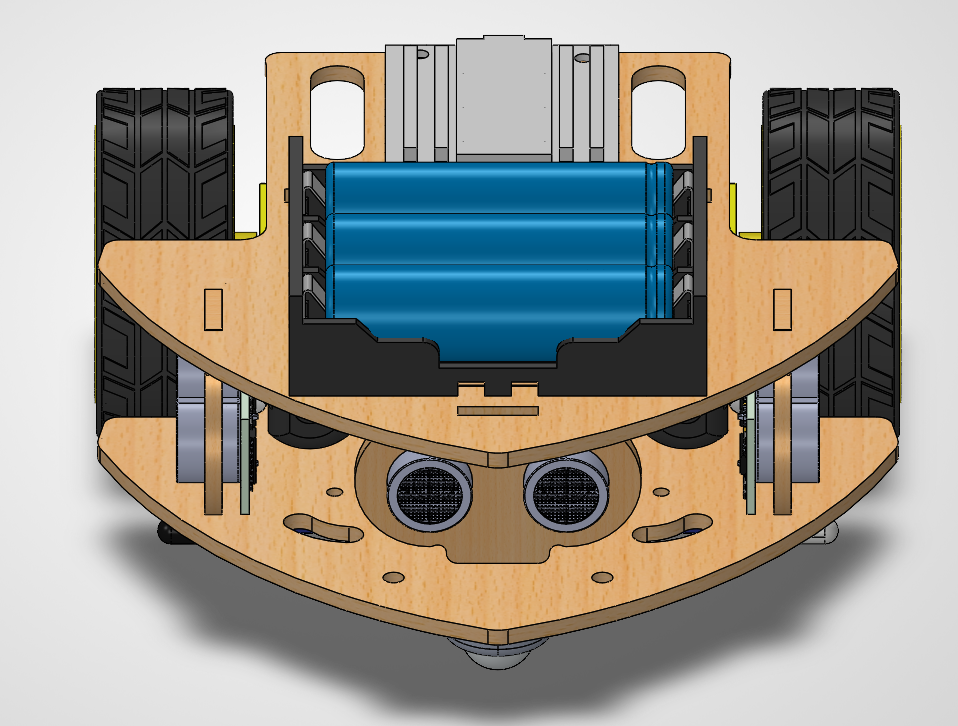
\includegraphics[width=0.62\columnwidth]{cad_1}\\[0.5em]
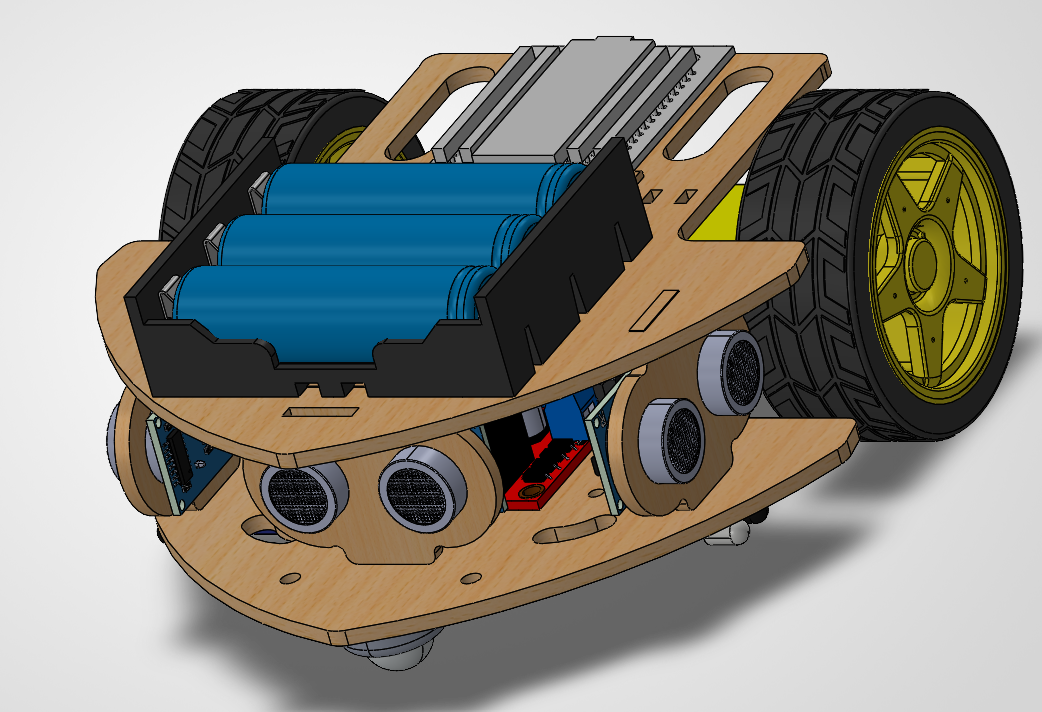
\includegraphics[width=0.62\columnwidth]{cad_2}
\caption{Modelo CAD del robot móvil: dos vistas del diseño.}
\label{fig:cad}
\end{figure}

La Fig.~\ref{fig:montaje} muestra el montaje real sobre la pista con líneas de colores.

\begin{figure*}[t]
\centering
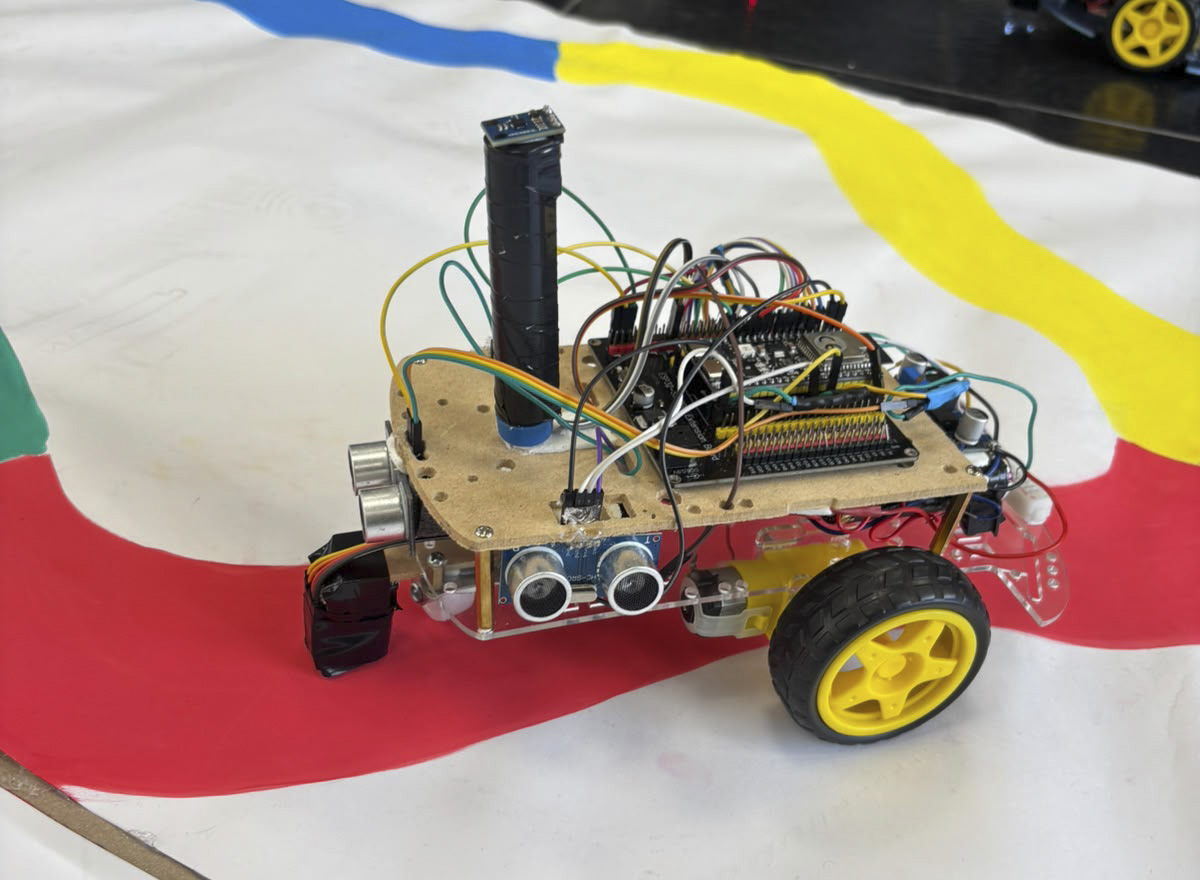
\includegraphics[width=0.56\textwidth]{montaje}
\caption{Montaje completo del robot sobre la pista con líneas de colores.}
\label{fig:montaje}
\end{figure*}

\section{Diseño electrónico}

\subsection{Alimentación}

La alimentación parte de una batería Li-ion 3S con BMS, interruptor y fusible, y dos convertidores: $6~\mathrm{V}$ para motores y $5~\mathrm{V}$ para lógica. La tierra es común entre batería, controlador, ESP32-S3 y sensores.

\subsection{Controlador de motores}

El PWM trabaja a $20~\mathrm{kHz}$ con 8 bits. STBY (GPIO18) permanece en bajo al arrancar y ante una emergencia. El sentido y el balance de las ruedas se corrigieron por software: el motor izquierdo está invertido y recibe 8 puntos porcentuales menos.

\subsection{Adaptación de señal de los ultrasonidos}

La salida ECHO entrega $5~\mathrm{V}$. Por eso cada sensor lleva un divisor de $R_1=1~\mathrm{k}\Omega$ y $R_2=2~\mathrm{k}\Omega$:

\begin{equation}
V_{\mathrm{GPIO}} = V_{\mathrm{ECHO}}\frac{R_2}{R_1+R_2}=5\cdot\frac{2}{3}\approx 3{,}33~\mathrm{V}
\label{eq:divisor}
\end{equation}

\section{Asignación de pines}

La Tabla~\ref{tab:pinout} contiene la asignación definida en \texttt{Config.h}. El QMC5883L (\texttt{0x0D}) y el TCS34725 (\texttt{0x29}) comparten el bus I2C, a $100~\mathrm{kHz}$.

\begin{table}[H]
\centering
\caption{Asignación de pines del ESP32-S3}
\label{tab:pinout}
\scriptsize
\begin{tabular}{l l}
\toprule
\textbf{Señal} & \textbf{GPIO} \\
\midrule
I2C SDA / SCL & 8 / 9 \\
HC-SR04 frontal TRIG / ECHO & 40 / 41 \\
HC-SR04 izquierdo TRIG / ECHO & 38 / 39 \\
HC-SR04 derecho TRIG / ECHO & 10 / 11 \\
Motor izquierdo IN1 / IN2 / PWM & 4 / 5 / 6 \\
Motor derecho IN1 / IN2 / PWM & 7 / 15 / 16 \\
TB6612FNG STBY & 18 \\
Encoder izquierdo A / B (reservados) & 12 / 13 \\
Encoder derecho A / B (reservados) & 14 / 21 \\
Parada de emergencia & 47 \\
\bottomrule
\end{tabular}
\end{table}

\section{Desarrollo del firmware}

\subsection{Entorno de desarrollo}

El firmware v0.4.0-nav está escrito en C++ con Arduino para ESP32 \cite{ArduinoESP32} y \texttt{arduino-cli}:

\begin{lstlisting}[basicstyle=\ttfamily\scriptsize,breaklines=true]
esp32:esp32:esp32s3:PSRAM=opi
\end{lstlisting}

\subsection{Organización por módulos}

\begin{itemize}
    \item \texttt{Config}, \texttt{Geometry}, \texttt{Diagnostics}: parámetros, cálculo de ángulos y diagnóstico.
    \item \texttt{MotorDriver}, \texttt{ControlManual}: potencia, consignas y caducidad.
    \item \texttt{Compass}, \texttt{ColorSensor}, \texttt{ObstacleSensor}, \texttt{Encoder}: sensores.
    \item \texttt{FSMGlobal}: modos y parada de emergencia.
    \item \texttt{Navigator}: navegación autónoma.
    \item \texttt{Protocol}, \texttt{Wireless}, \texttt{Telemetry}: comunicación.
\end{itemize}

\subsection{Temporización}

La brújula se lee cada $50~\mathrm{ms}$ y el color cada $120~\mathrm{ms}$. Los ultrasonidos se disparan uno cada $30~\mathrm{ms}$ para que no interfieran entre sí, y el ECHO se mide por interrupción. El módulo \texttt{Navigator} decide cada $50~\mathrm{ms}$.

\subsection{Seguridad}

El firmware incluye cuatro mecanismos: arranque con STBY en bajo; caducidad de $500~\mathrm{ms}$ en las órdenes manuales por WebSocket; validez de $200~\mathrm{ms}$ en cada consigna autónoma; y parada de emergencia enclavada, por aplicación, voz o pulsador.

\section{Comunicación inalámbrica y aplicación}

\subsection{Enlace y mensajes}

El robot crea la red \texttt{robot-esp32s3} y un servidor WebSocket en el puerto 81. La Tabla~\ref{tab:mensajes} resume los mensajes. Los inválidos se rechazan con códigos como \texttt{BAD\_FORMAT}, \texttt{UNSUPPORTED}, \texttt{SAFETY} o \texttt{VERSION\_MISMATCH}.

\begin{table}[H]
\centering
\caption{Mensajes principales del protocolo}
\label{tab:mensajes}
\scriptsize
\begin{tabular}{p{0.27\columnwidth} p{0.61\columnwidth}}
\toprule
\textbf{Mensaje} & \textbf{Función} \\
\midrule
\texttt{hello}, \texttt{ping}, \texttt{status} & Iniciar, comprobar el enlace y pedir estado. \\
\texttt{mode} & Elegir manual o autónomo, con submodo \texttt{evadir}, \texttt{rumbo} o \texttt{linea}. \\
\texttt{drive} & Mover o detener. \\
\texttt{heading} & Fijar el rumbo deseado. \\
\texttt{estop} & Parada de emergencia. \\
\texttt{telemetry} & Enviar sensores, motores, modo y navegación. \\
\texttt{ack}, \texttt{event}, \texttt{error} & Confirmar, avisar y rechazar. \\
\bottomrule
\end{tabular}
\end{table}

\subsection{Interfaz}

La interfaz está hecha en HTML y JavaScript y se sirve con Streamlit. En la Fig.~\ref{fig:interfaz} se ven la selección de modo, la conducción, las tres distancias, la brújula con el rumbo actual y el deseado, los motores, el color y la parada de emergencia. También tiene un modo simulación para usarla sin robot, en el que se tomaron las capturas.

\begin{figure*}[t]
\centering
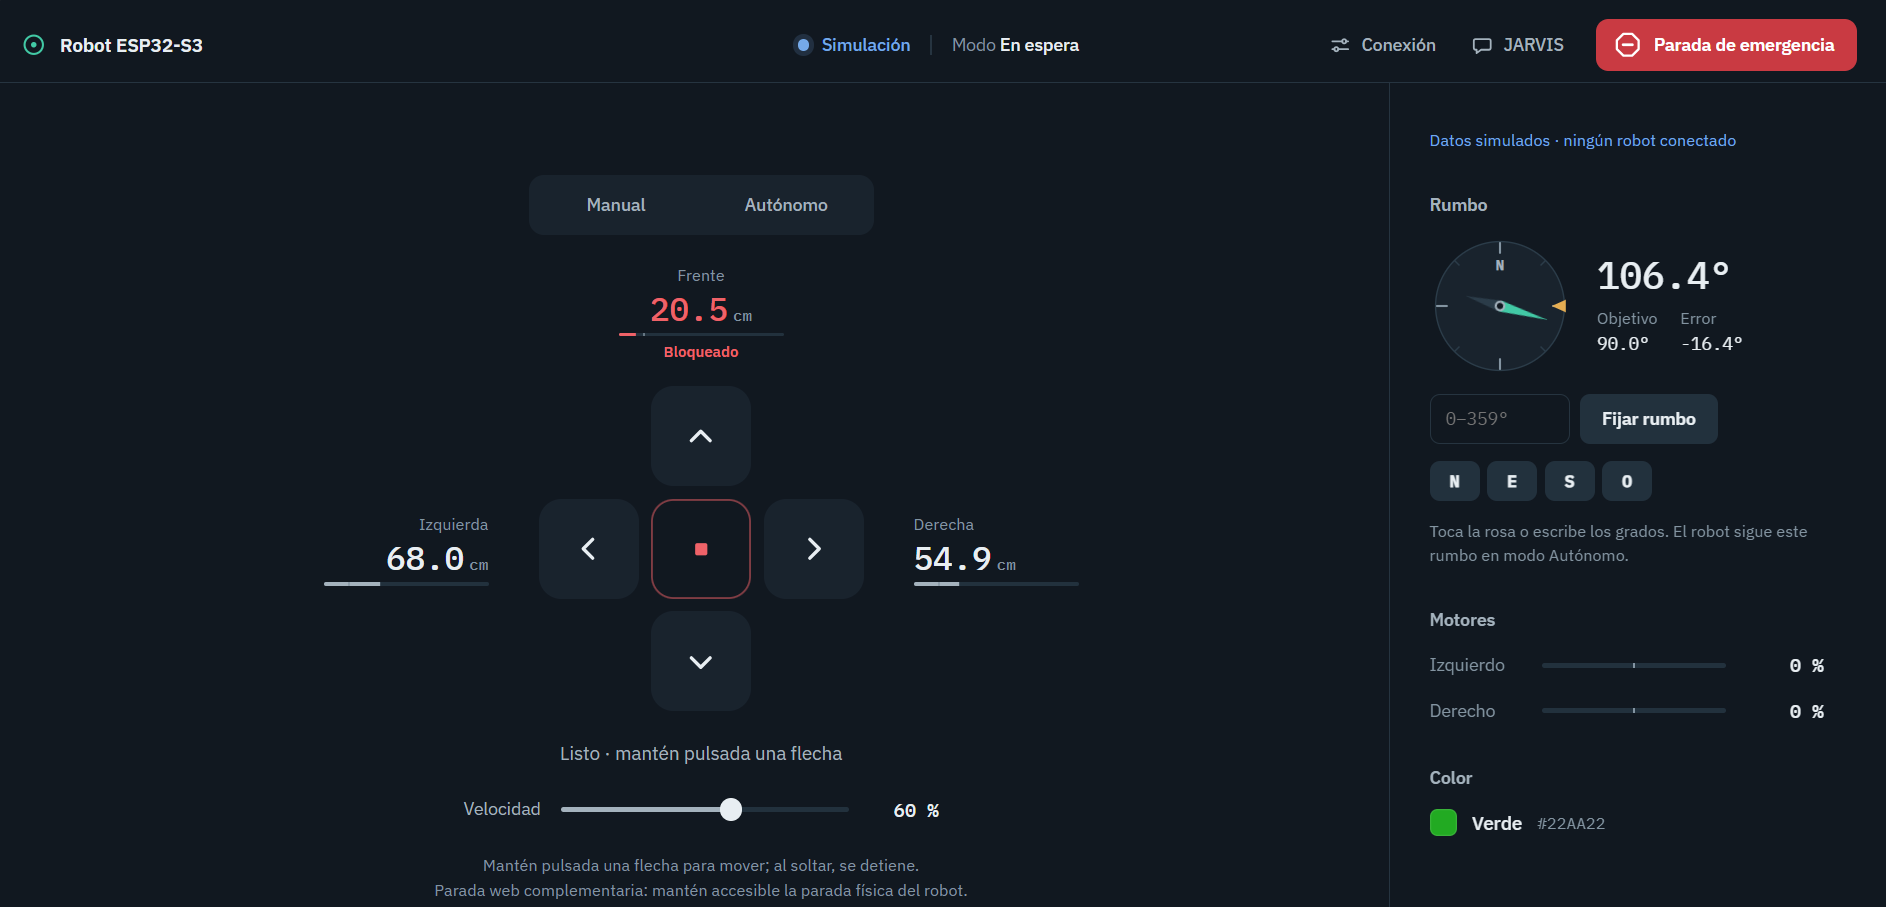
\includegraphics[width=0.60\textwidth]{interfaz}
\caption{Interfaz de control y telemetría (modo simulación).}
\label{fig:interfaz}
\end{figure*}

\section{Control manual y navegación autónoma}

\subsection{Control manual}

El robot se mueve mientras se mantiene pulsada una flecha y se detiene al soltarla. La conducción se bloquea sin enlace, en emergencia o en modo autónomo, pero la detención siempre está disponible.

\subsection{Control por voz}

La voz se reconoce con la Web Speech API y la frase se convierte en una orden, por ejemplo ``avanza'', ``rumbo 90'' o ``sigue la línea''. La parada tiene prioridad y las negaciones como ``no avances'' se ignoran.

\subsection{Submodos autónomos}

Al elegir el modo autónomo, la aplicación pide uno de los submodos de la Tabla~\ref{tab:submodos}; el robot no arranca sin él. Si la orden es por voz, JARVIS pregunta cuál usar.

\begin{table}[H]
\centering
\caption{Submodos autónomos}
\label{tab:submodos}
\scriptsize
\begin{tabular}{p{0.17\columnwidth} p{0.40\columnwidth} p{0.29\columnwidth}}
\toprule
\textbf{Submodo} & \textbf{Comportamiento} & \textbf{Tras el obstáculo} \\
\midrule
Solo esquivar & Avanzar recto & Sigue recto \\
Rumbo & Mantener el rumbo dado con la brújula & Recupera el rumbo \\
Línea & Seguir cualquier color distinto de blanco & Vuelve a la línea \\
\bottomrule
\end{tabular}
\end{table}

\subsection{Control de orientación}

El rumbo se corrige con un control proporcional sobre el error de la Ec.~\ref{eq:error_angular}:

\begin{equation}
u=\operatorname{sat}_{\pm 30}(0{,}8\,e_\theta),\quad
V_L=45+u,\quad V_R=45-u
\label{eq:control}
\end{equation}

con $V_L$, $V_R$ y $u$ en porcentaje. Si $|e_\theta|>45^\circ$, el robot gira en el sitio. Si la brújula falla, sigue avanzando y esquivando hasta recuperarla.

\subsection{Evasión de obstáculos}

Un obstáculo se detecta a menos de $25~\mathrm{cm}$. El robot gira hacia el lado con más espacio, lo bordea y retoma su tarea (Fig.~\ref{fig:evasion}). Si los tres sensores están bloqueados, retrocede $400~\mathrm{ms}$ y vuelve a decidir.

\begin{figure}[H]
\centering
\begin{tikzpicture}[
    st/.style={draw,rounded corners,align=center,minimum height=0.6cm,minimum width=1.85cm,font=\scriptsize},
    ar/.style={-{Latex[length=1.8mm]},thick}
]
\node[st] (n) at (0,0) {NAVEGAR};
\node[st] (e) at (2.9,0) {EVADIR};
\node[st] (b) at (5.8,0) {BORDEAR};
\node[st] (r) at (2.9,-1.2) {REORIENTAR};
\node[st] (v) at (5.8,-2.4) {VOLVER};
\node[st] (a) at (2.9,-2.4) {ALINEAR};
\draw[ar] (n) -- node[above,font=\tiny]{obstáculo} (e);
\draw[ar] (e) -- node[above,font=\tiny]{libre} (b);
\draw[ar] (b) to[out=135,in=45] node[above,font=\tiny]{solo esquivar} (n);
\draw[ar] (b.south west) -- node[below right,font=\tiny,pos=0.45]{rumbo} (r.east);
\draw[ar] (r.west) -- (n.south east);
\draw[ar] (b.south) -- node[right,font=\tiny]{línea} (v.north);
\draw[ar] (v) -- (a);
\draw[ar] (a.west) -| (n.south);
\end{tikzpicture}
\caption{Evasión y retorno según el submodo.}
\label{fig:evasion}
\end{figure}

\subsection{Seguimiento de línea}

El robot sigue el borde de la línea con un solo sensor: sobre color pivota alejándose al 70\,\% y sobre blanco vuelve al 55\,\%. Si ve blanco por más de $400~\mathrm{ms}$, busca la línea con barridos cada vez más amplios.

En la pista este fue el submodo más difícil, porque la búsqueda de la línea resultó muy deficiente en las curvas. El robot sí reconocía los colores; el problema era que giraba bastante rápido mientras buscaba y el sensor, que entrega una lectura cada $120~\mathrm{ms}$, se demoraba en leer. Así pasaba sobre la línea sin detectarla y se perdía.

\subsection{Detección de seis colores}

El TCS34725 trabaja con ganancia 16x e integración de $103~\mathrm{ms}$. Durante la calibración tuvimos un problema: la luz ambiente alteraba las lecturas y un mismo color daba valores distintos. Lo solucionamos con cinta aislante en el borde del sensor, para bloquear la luz externa, y redujimos el espacio entre el sensor y la superficie, con lo que la lectura mejoró.

Para la calibración tomamos 450 muestras, 75 por color en tres posiciones, y obtuvimos un 100\,\% de aciertos. La Tabla~\ref{tab:color} presenta los promedios.

\begin{table}[H]
\centering
\caption{Promedios de calibración del TCS34725 (75 muestras por color)}
\label{tab:color}
\scriptsize
\begin{tabular}{lccc}
\toprule
\textbf{Color} & \textbf{RGB promedio} & \textbf{Clear} & \textbf{Aciertos} \\
\midrule
Negro & (1501, 1273, 703) & 3595 & 75/75 \\
Blanco & (9090, 6934, 4169) & 20733 & 75/75 \\
Rojo & (7092, 1480, 1168) & 9456 & 75/75 \\
Amarillo & (9700, 6802, 2374) & 19528 & 75/75 \\
Verde & (1281, 2291, 1210) & 4882 & 75/75 \\
Azul & (1051, 1665, 1920) & 4632 & 75/75 \\
\bottomrule
\end{tabular}
\end{table}

\section{Asistente JARVIS}

JARVIS funciona con reglas, sin depender de un modelo de lenguaje externo. El botón ``Hablar'' sirve tanto para preguntarle como para dar órdenes, y la respuesta siempre es hablada (Fig.~\ref{fig:jarvis}). Su base técnica reúne 20 temas sobre alimentación, conexiones, temporizadores, sensores, comunicación, seguridad y navegación. Para los valores actuales, JARVIS lee la telemetría.

\begin{figure*}[t]
\centering
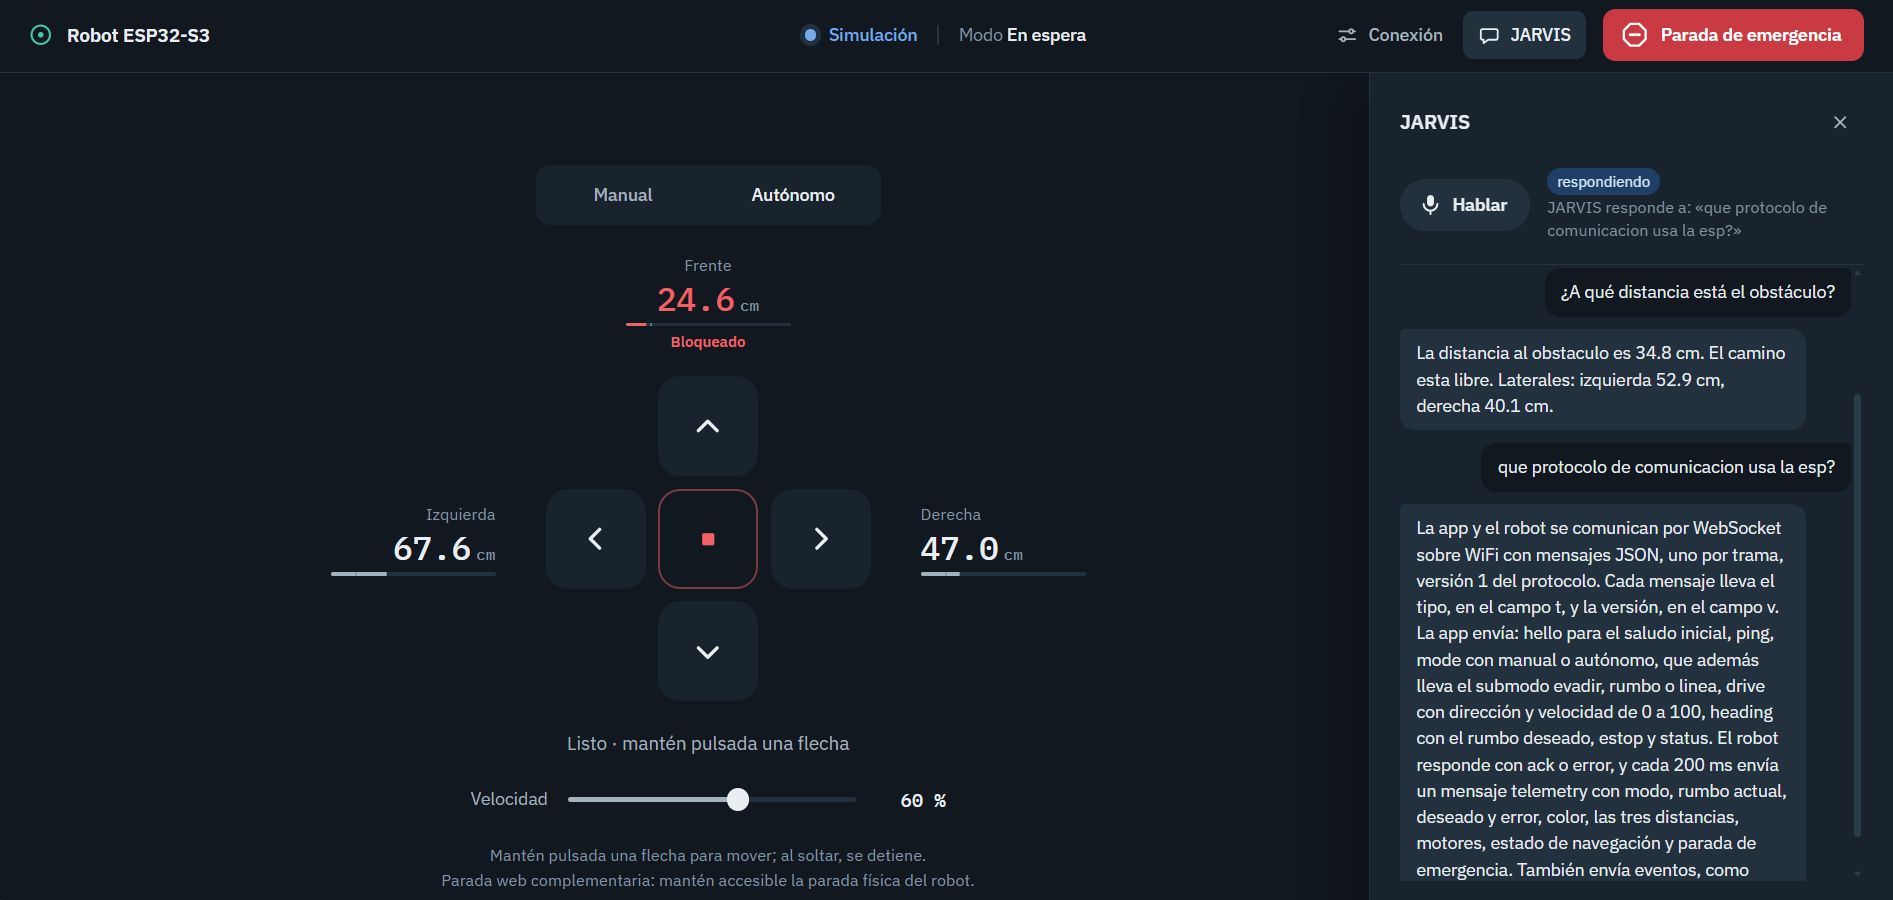
\includegraphics[width=0.60\textwidth]{interfaz_jarvis}
\caption{Interfaz con el asistente JARVIS respondiendo una pregunta técnica (modo simulación).}
\label{fig:jarvis}
\end{figure*}

\section{Metodología}

\begin{enumerate}[1.]
    \item \textbf{Análisis:} definición de requisitos y arquitectura.
    \item \textbf{Diseño:} selección de componentes, modelo del chasis y asignación de pines.
    \item \textbf{Desarrollo:} firmware, protocolo, aplicación, voz y JARVIS.
    \item \textbf{Pruebas de software:} verificación de la lógica en el PC y simulación de la navegación.
    \item \textbf{Integración:} montaje, prueba de motores, calibración del color y conexión con la aplicación.
    \item \textbf{Validación:} pruebas de sensores, voz, JARVIS y los tres submodos en el robot.
\end{enumerate}

\section{Resultados}

\subsection{Compilación del firmware}

El firmware v0.4.0-nav compila para el ESP32-S3 y ocupa 1\,058\,414 bytes, el 80\,\% de la memoria de programa.

\subsection{Pruebas de software}

Las nueve pruebas de la Tabla~\ref{tab:pruebas} terminaron sin fallos.

\begin{table}[H]
\centering
\caption{Pruebas de software (9 de 9 sin fallos)}
\label{tab:pruebas}
\scriptsize
\begin{tabular}{p{0.36\columnwidth} p{0.52\columnwidth}}
\toprule
\textbf{Prueba} & \textbf{Alcance} \\
\midrule
Error angular & Intervalo y giro más corto. \\
Color & Clasificación con lecturas reales. \\
Obstáculos & Conversión y disparo escalonado. \\
Navegación & Submodos, evasión y retorno. \\
Aplicación Streamlit & Voz y JARVIS del panel nativo. \\
Protocolo & Validación en ambos sentidos. \\
Comandos & Voz o texto a orden. \\
JARVIS & Preguntas, órdenes y respuestas. \\
Integración WebSocket & Enlace, caducidad y emergencia con robot simulado. \\
\bottomrule
\end{tabular}
\end{table}

\subsection{Simulación de la navegación}

En simulación geométrica, con una línea recta y cajas de 8, 12 y $16~\mathrm{cm}$ a ambos lados, el robot rodea el obstáculo y vuelve a la línea sin colisiones. Este caso no incluye obstáculos en curva.

\subsection{Precisión de las distancias}

La medición de los ultrasonidos se comprobó con un pie de rey en distancias cortas, donde el desfase fue de aproximadamente $2~\mathrm{mm}$. Las distancias mayores a $20~\mathrm{cm}$ se midieron con un metro y el desfase fue de aproximadamente $2~\mathrm{cm}$.

\subsection{Seguimiento de línea en curvas}

Hicimos 20 pruebas en curvas y el robot se perdió en 16 de ellas, es decir, en el 80\,\%. Solo en 4 (20\,\%) completó la curva.

\subsection{Pruebas en el robot}

La Tabla~\ref{tab:robot} resume las pruebas en el prototipo.

\begin{table}[H]
\centering
\caption{Resultados en el robot}
\label{tab:robot}
\scriptsize
\begin{tabular}{p{0.50\columnwidth} p{0.38\columnwidth}}
\toprule
\textbf{Elemento} & \textbf{Resultado} \\
\midrule
Motores: sentido, PWM, STBY y caducidad & Pasa (banco) \\
Color: 450 muestras & 100\,\% de aciertos \\
Brújula QMC5883L & Funciona \\
Tres HC-SR04 & Funcionan; desfase de 2 mm (corta) y 2 cm ($>$20 cm) \\
Comunicación aplicación--robot & Funciona \\
Control por voz & Funciona \\
JARVIS & Funciona \\
Submodo solo esquivar & Funciona \\
Submodo rumbo & Funciona \\
Submodo línea & Funciona; se pierde en 16 de 20 pruebas en curva \\
\bottomrule
\end{tabular}
\end{table}

\section{Limitaciones y problemas encontrados}

\begin{itemize}
    \item La búsqueda de la línea es deficiente en las curvas: el robot gira muy rápido para el tiempo de lectura del sensor y se perdió en el 80\,\% de las pruebas.
    \item La luz ambiente afectaba la lectura de color; la cinta aislante y la menor distancia a la superficie redujeron el problema.
    \item El desfase de los ultrasonidos aumenta con la distancia.
    \item La pérdida de Wi-Fi no detiene el modo autónomo; la caducidad de $500~\mathrm{ms}$ protege el modo manual.
    \item La prueba del pulsador físico de emergencia sigue pendiente.
\end{itemize}

\section{Conclusiones}

\begin{itemize}
    \item Logramos un robot funcional que integra sensores, motores, comunicación y supervisión con un ESP32-S3.
    \item Los tres submodos autónomos funcionaron en el robot. El de línea fue el más difícil: se perdió en 16 de 20 pruebas en curva, no por confundir los colores, sino porque giraba más rápido de lo que el sensor podía leer.
    \item La lectura de color depende mucho de la luz ambiente y de la altura del sensor. Con la cinta aislante y menos espacio hasta la superficie obtuvimos un 100\,\% de aciertos en 450 muestras.
    \item Los ultrasonidos son precisos a corta distancia, con un desfase de unos 2~mm, suficiente para detectar obstáculos a 25~cm aun con el desfase de 2~cm que aparece a mayor distancia.
    \item Reunir en un mismo botón las preguntas a JARVIS y las órdenes de voz hizo más sencillo el uso del robot.
\end{itemize}

\section{Trabajo futuro}

\begin{enumerate}[1.]
    \item Reducir la velocidad de giro en la búsqueda y acortar el tiempo de lectura del color.
    \item Agregar más sensores de color para no perder la línea en las curvas.
    \item Compensar el desfase de los ultrasonidos a distancias mayores.
    \item Detener el modo autónomo ante la pérdida de Wi-Fi.
    \item Probar el pulsador físico de emergencia.
\end{enumerate}

\section{Repositorio del proyecto}

El código y la documentación están en:

\begin{center}
\url{https://github.com/kevinparra943/robot-movil-esp32s3}
\end{center}

\ifCLASSOPTIONcaptionsoff
  \newpage
\fi

\begin{thebibliography}{11}

\bibitem{Espressif}
Espressif Systems, ``ESP32 Series Datasheet,'' documentación técnica del microcontrolador ESP32. Disponible en: \url{https://www.espressif.com/en/support/documents/technical-documents}

\bibitem{ArduinoESP32}
Espressif Systems, ``Arduino-ESP32 Documentation,'' documentación del framework Arduino para ESP32. Disponible en: \url{https://docs.espressif.com/projects/arduino-esp32/en/latest/}

\bibitem{TB6612}
Toshiba Electronic Devices \& Storage Corporation, ``TB6612FNG Dual DC Motor Driver IC,'' hoja de datos del controlador de motores.

\bibitem{QMC5883L}
QST Corporation, ``QMC5883L 3-Axis Magnetic Sensor,'' documentación técnica del magnetómetro.

\bibitem{TCS34725}
ams OSRAM, ``TCS3472 Color Light-to-Digital Converter,'' hoja de datos del sensor de color. Disponible en: \url{https://ams-osram.com/}

\bibitem{HCSR04}
ElecFreaks, ``HC-SR04 Ultrasonic Ranging Module,'' documentación técnica del módulo ultrasónico.

\bibitem{WebSocket}
I. Fette y A. Melnikov, ``The WebSocket Protocol,'' RFC 6455, Internet Engineering Task Force, 2011. Disponible en: \url{https://www.rfc-editor.org/rfc/rfc6455}

\bibitem{JSON}
T. Bray, Ed., ``The JavaScript Object Notation (JSON) Data Interchange Format,'' RFC 8259, Internet Engineering Task Force, 2017. Disponible en: \url{https://www.rfc-editor.org/rfc/rfc8259}

\bibitem{MDN}
Mozilla Foundation, ``MDN Web Docs: WebSocket API,'' documentación técnica. Disponible en: \url{https://developer.mozilla.org/docs/Web/API/WebSocket}

\bibitem{Siegwart}
R. Siegwart, I. R. Nourbakhsh y D. Scaramuzza, \emph{Introduction to Autonomous Mobile Robots}, 2a. ed. Cambridge, MA, EUA: MIT Press, 2011.

\end{thebibliography}

\end{document}
